\documentclass{article}
\usepackage{hyperref,graphicx}

\title{Base di Dati 1}
\author{Riccardo Cara}

\begin{document}
\maketitle

\tableofcontents
\newpage

\section{Introduzione ai database e ai DBMS}

    Un \textit{database} o Base di Dati è un insieme di dati organizzati in \textit{strutture dati}, esse ne facilitano la creazione, l'accesso e l'aggiornamento.
    I dati possono essere:

    \begin{itemize}
        \item \textbf{dati strutturati}:
        oggetti rappresentati da piccole stringhe di simboli o numeri

        \item \textbf{dati non strutturati:}
        testo scritto in linguaggio umano
        \end{itemize}

    I dati all'interno di un Database vengono gestiti tramite un Database Management System o DBSM ossia il software per la gestione di grandi masse di dati condivise, strutturate e processabili, residenti su una memoria.

    \paragraph{Informazione strutturata} la struttura dell'informazione dipende dal suo utilizzo e può essere modificata nel tempo, facendo un esempio, se si volessero archiviare i dati di una persona, avremmo:
    \begin{itemize}
        \item{nome}
        \item{cognome}
        \item{data di nascita}
        \item{luogo di nascita}
    \end{itemize}
    L'obbiettivo è di facilitare l'elaborazione dei dati sulla base delle loro relazioni che vengono rappresentate tramite record\label{word:record}:

    \begin{center}
    \begin{tabular}{|c|c|c|c|c|}
        \hline 
        \textbf{nome} & \textbf{cognome} & \textbf{data di nascita}& \textbf{luogo di nascita} \\
        \hline
        Francesco & Totti & 27/09/1976& Roma\\
        \hline
    \end{tabular}
    \end{center}
    per accedere ai dati individuali nella struttura dati, vengono fatte delle "interrogazioni" o \textit{query}. Un database è una risorsa condivisa tra diverse componenti in un organizzazione, quando più componenti vogliono accedere allo stesso dato contemporaneamente si crea un problema di \hyperref[sec:concorrenza]{concorrenza} che comporta la necessità di gestire gli accessi contemporanei agli stessi dati.
\section{Sistema Informativo}
    Un \textit{sistema informativo} è concettualmente organizzato in aggregati di informazioni omogenee (file \footnote{esistono alcuni sottofile chiamati indici che permettono di recuperare velocemente le informazioni dai file principali}), gli aggregati sono le componenti del sistema informativo. Un operazione di aggiornamento ha per oggetto un singolo aggregato, mentre una query può coinvolgerne molteplici.

    \subsection{Livelli di astrazione}
        Un database ha tre livelli di astrazione:
        %
        \begin{itemize}
            \item \textbf{schema esterno}:
            descrizione di una porzione del database tramite un modello logico che può differire dallo schema logico e rispecchia i bisogni e privilegi di accesso di diversi tipi di utente, l'accesso al database avviene solamente tramite lo schema esterno

            \item \textbf{schema logico}:
            descrizione dell'intero database nel "principale" modello logico del DBMS

            \item \textbf{schema fisico}:
            rappresentazione dello schema logico sulle strutture di archiviazione fisica
        \end{itemize}
        %
        quando si parla di schema e istanze, con schema si intende in una tabella, la prima riga che definisce il tipo di dato
        %
            \begin{tabular}{|c|c|c|}
            \hline
                nome &cognome& data di nascita \\
            \hline
            \end{tabular}
        %
        con istanza si intende invece il "corpo" della tabella ovvero i valori correnti.
        %
    \subsection{Linguaggi per database}
        Esistono diversi linguaggi utilizzabili per creare/gestire database, DDL,DML,SQL.
        %
        \begin{itemize}
            \item \textbf{DDL}(Data Definition Language):
            per la definizioni di schemio logici, esterni, fisici e altre operazioni generali

            \item \textbf{DML}(Data Manipulation Language):
            per effettuare query e aggiornare le istanze

            \item \textbf{SQL}(Structured Query Language):
            è un linguaggio standardizzato per database basati su modelli relazionali che permette di fare entrambe le azioni del DDL e del DML
        \end{itemize}
        %
    \subsection{Modello di dati}
        Un modello è una struttura da utilizzare per organizzare i dati di interesse e le loro relazioni, un modello è composto da costruttori di tipo, ad esempio il modello relazionale prevede il costruttore di relazione (organizza in \hyperref[word:record]{record} i dati con una relazione). I modelli dei dati si dividono in due gruppi:
        %
        \begin{itemize}
            \item \textbf{modelli logici:}
            i modelli logici non dipendono da come vengono archiviati i dati fisicamente, ma disponibili secondo il modello tramite i DBMS.
            alcuni modelli logici sono: reticolare, gerarchico, relazionale, a oggetti.
            
            \item \textbf{modelli concettuali:}
            i modelli concettuali sono utilizzati all'inizio della progettazione di un database, essi non sono dipendenti dalle modalità di realizzazione, hanno lo scopo di rappresentare entità del mondo reale e le loro relazioni nelle prime fasi di pianificazione di un database, uno dei più utilizzati è il modello entità-relazione.
        \end{itemize}
        %
        vediamo tipi diversi di modelli dati:
        %
        \begin{itemize}

            \item \textbf{Modello Mesh}:
            Nel modello Mesh, i dati sono rappresentati in collezioni di record omogenei, le relazioni binarie vengono rappresentate come links, implementati come puntatori e quindi dipendenti dalla struttura fisica del database. È possibile rappresentare il modello graficamente:
            
            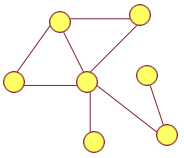
\includegraphics[]{immagini/modello Mesh.png}

            Il modello è rappresentato da nodi e linee. I nodi rappresentano i record e le linee che connettono i nodi rappresentano i links tra essi. Il modello più popolare di modello mesh è \textit{CODASYL}

            \item \textbf{Modello gerarchico}:
            il modello gerarchico è un tipo di modello mesh in cui i collegamenti fra i nodi vengono fatti in maniera gerarchica, i nodi hanno quindi forma di albero e hanno come padre un solo nodo
            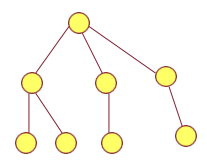
\includegraphics[]{immagini/modello gerarchico.png}

            \item \textbf{modello relazionale}:
            i dati e le relazioni sono rappresentate da valori, non ci sono riferimenti espliciti come i puntatori nei modelli mesh o gerarchici. Gli oggetti del mondo reale sono rappresentati come record in cui i campi sono sono riempiti da informazioni di interesse (nome, cognome, data di nascita).

            \item \textbf{modello a oggetti}:
            è un modello basato su oggetti (persona, macchina, animale), gli attributi descrivono lo stato dell'oggetto
        \end{itemize}
        %
    \subsection{Modello relazionale}
        È già stato definito il Modello relazionale nella precedente sezione, si vuole ora approfondire l'argomento.
        Il modello relazionale si basa sulla nozione matematica di relazione. Si definisce con \textit{dominio} (D) un insieme di valori, un sottoinsieme del prodotto cartesiano di k domini $D_1\times D_2 \times ...\times D_k$ ha nome di \textit{relazione matematica}, introduciamo due definizioni.
        
        \begin{itemize}
            \item \textbf{grado}:
                con grado k si intende la relazione matematica di k domini.

            \item \textbf{attributo}:
                un attributo è definito da un nome A e dal suo dominio dom(A)

                \begin{tabular}{|c|}
                    \hline
                    \textbf{nome}\\
                    \hline
                    Nerone\\
                    \hline

                \end{tabular}
                
                in cui $A=nome$, $dom(A)=str$ e l'attributo è l'insieme di questi.
            
            \item \textbf{schema}:
                Un insieme di attributi è detto schema, lo schema relazionale viene scritto come $R(A_1,A_2,...,A_k)$, descrive la sua struttura ed è invariante nel tempo.
            
            \item \textbf{istanza}:
                l'instanza $r$ contiene tutti i valori correnti in una relazione $R$. 

            \item \textbf{n-upla}:
                una n-upla è un elemento della relazione (un elemento è la riga di una tabella), il numero di n-uple di una relazione è chiamata cardinalità. In ogni n-upla della relazione di ordine k, i componenti della n-upla sono ordinati secondo k, dati $D_1$,$D_2$,...,$D_k$, gli attributi saranno:

                \begin{tabular}{|c |c |c |c|}
                    \hline
                    $attributo_1$&$attributo_2$&$...$&$attributo_k$\\
                    \hline
                \end{tabular}
                
                una n-upla da un punto di vista matematico, è una funzione definita in $R$(relazione) che associa ogni attributo A in R ad un elemento del dominio $dom(a)$, il valore dell'attributo A equivale a $t[A]$ in cui t è tupla/n-upla.

            \item \textbf{tabella}:
                una tabella è l'insieme delle n-uple di una relazione.
            \item \textbf{schema del database}:
                lo schema del database è un insieme di schemi relazionali. Lo schema di un database relazionale è un insieme $R_1,R_2,...,R_n$ degli schemi. Un database relazionale è l'insieme $r_1,r_2,...,r_n$ in cui $r_1$ è l'istanza di $R_1$.
                
                \paragraph{esempio}
                    schema: info città (città,regione,popolazione)
                    
                    istanza:
                    \begin{tabular}{|c|c|c|}
                        \hline
                        Roma & Lazio & 3000000\\
                        \hline
                        Milano &Lombardia & 1500000\\
                        \hline
                        Genova & Liguria& 800000\\
                        \hline
                        Pisa & Toscana & 150000\\
                        \hline
                    \end{tabular}
            
            
        \end{itemize}

        \paragraph{esempio}:
            definendo $k=2$ e $D_1=\{bianco,nero\},D_2=\{0,1,2\}$, il prodotto cartesiano sarà $D_1\times D_2=\{(bianco,0),(bianco,1),(bianco,2),(nero,0),(nero,1),(nero,2)\}$, è possibile ora definire una relazione, un esempio di relazione è $\{(bianco,0),(bianco,2),(nero,1)\}$ ovvero una relazione di grado 2 con cardinalità 3.

\section{Algebra Relazionale}

\section{Teoria Relazionale}

\section{Organizzazione Fisica}

\section{Concorrenza} \label{sec:concorrenza}


\end{document}
